\documentclass{beamer}

\usepackage{subfigure}
\renewcommand*{\subcapsize}{\tiny}
\usepackage[backend=bibtex]{biblatex}
\addbibresource{bib/main.bib}

\newcommand\fixme[2][FIXME]{\textcolor{red}{\textbf{#1:} #2}}
\usepackage[labelsep=space]{caption}
\usepackage[ruled, vlined, linesnumbered]{algorithm2e}

\SetKwInput{KwInput}{Input}
\SetKwInput{KwOutput}{Output}

\usepackage{amsmath}
\DeclareMathOperator*{\argmax}{arg\,max}

\usetheme[subsectionpage=progressbar, progressbar=frametitle]{metropolis}
\setbeamerfont{footnote}{size=\tiny}

\definecolor{turquoise}{RGB}{64,224,208}
\definecolor{turqbrown}{RGB}{92,80,60}
\setbeamercolor{progress bar}{fg=turquoise}
\setbeamercolor{normal text}{fg=turqbrown}
\title{Reinforcement Learning:\\ Basics, History, and Context}
\author{W. Cannon Lewis II}

\date{September 2, 2020}

\begin{document}
\begin{frame}
  \titlepage
\end{frame}

\section{Basics}
\begin{frame}{Introducing RL: Environment and Agent}
  \begin{figure}
    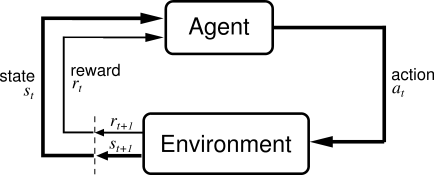
\includegraphics[keepaspectratio,width=\textwidth]{assets/agent_env}
  \end{figure}
\end{frame}

\begin{frame}{The Markov Assumption}
  \begin{itemize}
    \item We assume that the state $s_t$ and action $a_t$ contain all of the information needed to predict $s_{t+1}$. \\
    \item When does this hold in the real world? \\
    \item We call an environment with this property a \textbf{Markov Decision Process (MDP)}\footfullcite{puterman2014markov}
  \end{itemize}
\end{frame}

\begin{frame}{Example: Gridworld}
  \begin{figure}
    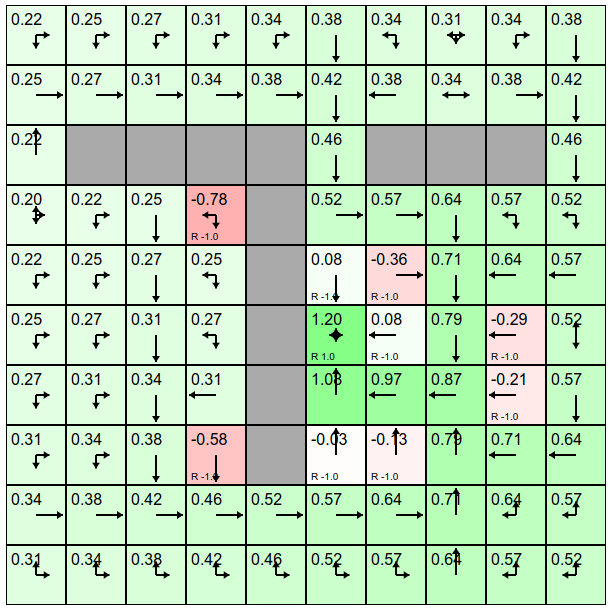
\includegraphics[keepaspectratio,width=0.5\textwidth]{assets/gridworld}
    \caption{\footnote{\url{https://cs.stanford.edu/people/karpathy/reinforcejs/}}}
  \end{figure}
\end{frame}

\begin{frame}{How Is RL Different from Other Kinds of Learning?}
  \begin{itemize}
    \item We must choose between \textbf{collecting informative data} and optimizing the \textbf{policy's performance}
    \item Benchmarking criteria are less clear---what are appropriate metrics for success?\footfullcite{Recht2019}
    \item In general, the distribution of data that we must learn from is \textbf{nonstationary} and \textbf{unbalanced}
  \end{itemize}
\end{frame}

\begin{frame}{Some Notation}
  \begin{itemize}
    \item $x_t \in X$ (or $s_t$) are states, $u_t \in U$ (or $a_t$) are actions. 
    \item $r_t \in \mathbb{R}$ is a reward given by a \emph{reward function} $R : X \times U \rightarrow \mathbb{R}$.
    \item $P: X \times U \rightarrow X$ is a transition function, which can be probabilistic.
    \item $\pi: X \rightarrow U$ is a \emph{policy} (or controller).
    \item $V_\pi: X \rightarrow \mathbb{R}$ and $Q_\pi: X \times U \rightarrow \mathbb{R}$ are \emph{value functions} which tell us how good a policy is in an environment.
  \end{itemize}
\end{frame}

\begin{frame}{Value Functions in RL}
  State value function\footfullcite{Sutton1998IntroductionTR}:
  \begin{equation}
    V_\pi(x) = \mathbb{E}\left[\sum_{t=0}^T \gamma^t R(x_t, \pi(x_t)) \mid x_0 = x\right]
  \end{equation}
  satisfies Bellman equation
  \begin{equation}
    V_\pi(x) = \mathbb{E}\left[R(x, \pi(x)) + \gamma V_\pi(x_{t+1})\right]
  \end{equation}
\end{frame}

\begin{frame}{A Basic Policy Iteration Algorithm}
  \begin{algorithm}[H]
      \DontPrintSemicolon
      \KwInput{An MDP $(X, U, R, P)$}
      \KwOutput{A policy $\pi$ optimizing rewards in the MDP}

      Initialize policy $\pi$ and $V_\pi$ \\
      \While {$\pi$ not stationary} {
        Estimate $V_\pi$ (\textbf{Policy Evaluation}) \\
        Set $\pi(x_t) = \argmax_{u_t} \left[r_t +  \gamma V_\pi(x_{t+1})\right]\ \forall x_t \in X$ \\ 
      }

      \textbf{Return} $\pi$

      \caption{Policy Iteration}
      \label{alg:stability_policy_iteration}
  \end{algorithm}
\end{frame}

\section{History}

\begin{frame}{Bellman and Dynamic Programming}
  \begin{columns}
    \begin{column}{0.48\textwidth}
      \begin{itemize}
        \item Invented dynamic programming for use on optimal control problems
        \item Coined the term ``Curse of Dimensionality''
      \end{itemize}
    \end{column}
    \begin{column}{0.48\textwidth}
      \begin{figure}
        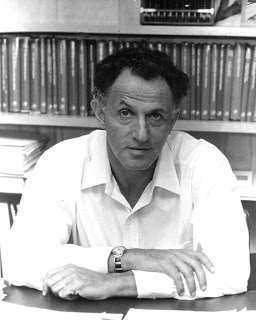
\includegraphics[keepaspectratio,width=0.5\textwidth]{assets/bellman}
      \end{figure}
    \end{column}
  \end{columns}
\end{frame}

\begin{frame}{Reinforcement Learning for Control}
  \begin{itemize}
    \item Classical reinforcement learning (e.g., Gridworld) $\neq$ RL for control
    \item Finite number of states and actions $\rightarrow$ uncountably many 
    \item Function approximation is often necessary\footfullcite{Bertsekas1996NeurodynamicP}
  \end{itemize}
\end{frame}

\begin{frame}{Optimal Control}
  ``Linear Quadratic Control'': Optimally control a system\footfullcite{hespanha2018linear} given by 
  \begin{align}
    x_{t+1} &= Ax_t + Bu_t + c + e_t \\
    u_t &= Kx_t + k
  \end{align}
  under a cost function
  \begin{equation}
    J(x_t, u_t) = x_t^\top Q x_t + u_t^\top R u_t
  \end{equation}
\end{frame}

\begin{frame}{A Multi-Field History: The HJB Equations}
  The Hamilton-Jacobi-Bellman equation is a PDE that gives rise to optimal
  controllers in continuous time problems:
  \begin{equation}
    \frac{\partial V(x, t)}{\partial t} + \min_u \left { \frac{\partial V(x, t)}{\partial x} \cdot F(x, u) + C(x, u) \right } = 0
  \end{equation}
  This equation is analogous to the Bellman equation for RL, and shows how RL
  sits at the intersection of physics, control, and artificial intelligence.
\end{frame}

\begin{frame}{Other RL-Adjacent Control}
  \begin{itemize}
    \item \textbf{Robust Control} computes controllers offline that are robust to certain kinds of uncertainty.
    \item \textbf{Adaptive Control} computes controllers that adapt to uncertainty online.
    \item \textbf{Dual Control} computes controllers that explicitly reduce uncertainty during execution.
  \end{itemize}
\end{frame}

\begin{frame}{Highlight: RL Bicycle Riding}
  \begin{columns}
    \begin{column}{0.3\textwidth}
      \begin{figure}
        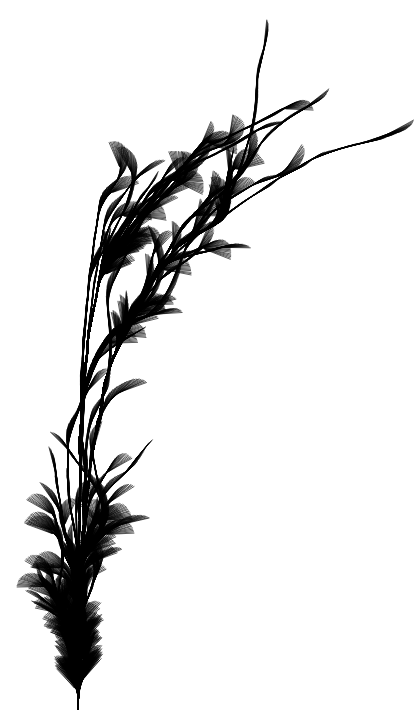
\includegraphics[width=0.9\textwidth]{assets/bicycle_1}
      \end{figure}
    \end{column}
    \begin{column}{0.65\textwidth}
      \begin{figure}
        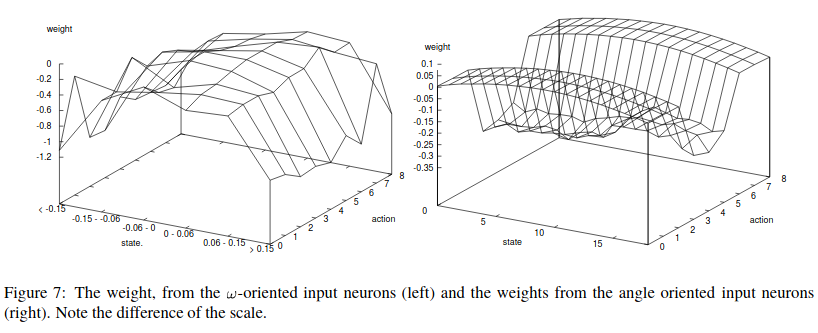
\includegraphics[width=\textwidth]{assets/bicycle_2}
      \end{figure}
    \end{column}
  \end{columns}\fullcite{Randlv1998LearningTD}
\end{frame}

\begin{frame}{Highlight: Inverted Helicopter Flight}
  \begin{columns}
    \begin{column}{0.3\textwidth}
      \begin{figure}
        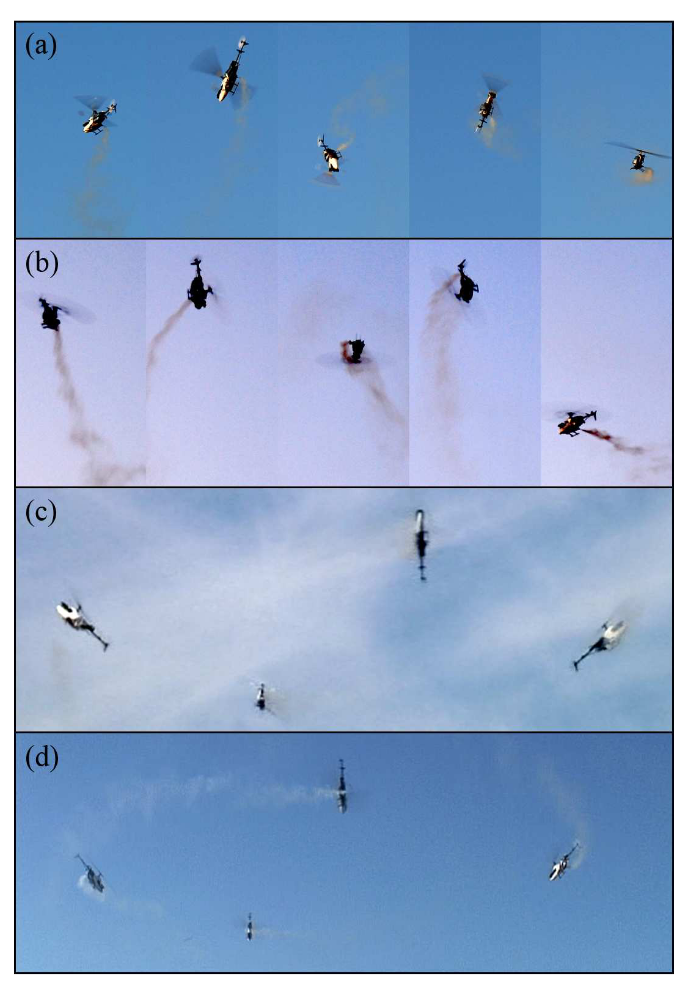
\includegraphics[width=0.9\textwidth]{assets/helicopter_2}
      \end{figure}
    \end{column}
    \begin{column}{0.65\textwidth}
      \begin{figure}
        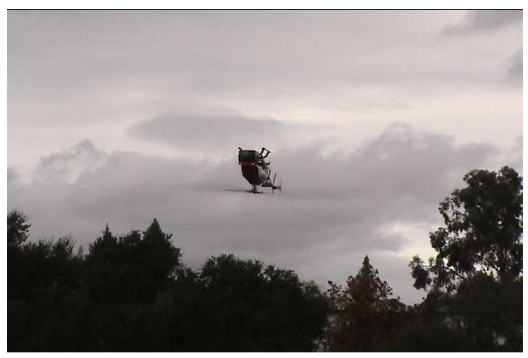
\includegraphics[width=\textwidth]{assets/helicopter_1}
      \end{figure}
    \end{column}
  \end{columns}\fullcite{Ng2003AutonomousHF}
\end{frame}

\section{Context}

\begin{frame}{What Happened in 2013?}
  \begin{itemize}
    \item Deepmind released and publicized \emph{Deep Q-Networks} (DQN)\footfullcite{Mnih2013PlayingAW}, which achieved new records on an Atari video game benchmark
    \item Spawned DDPG\footfullcite{lillicrap2015continuous}, PPO\footfullcite{Schulman2017ProximalPO}, and a whole host of other Deep RL methods.
  \end{itemize}
\end{frame}

\begin{frame}{So What is This Deep RL?}
  \begin{figure}
    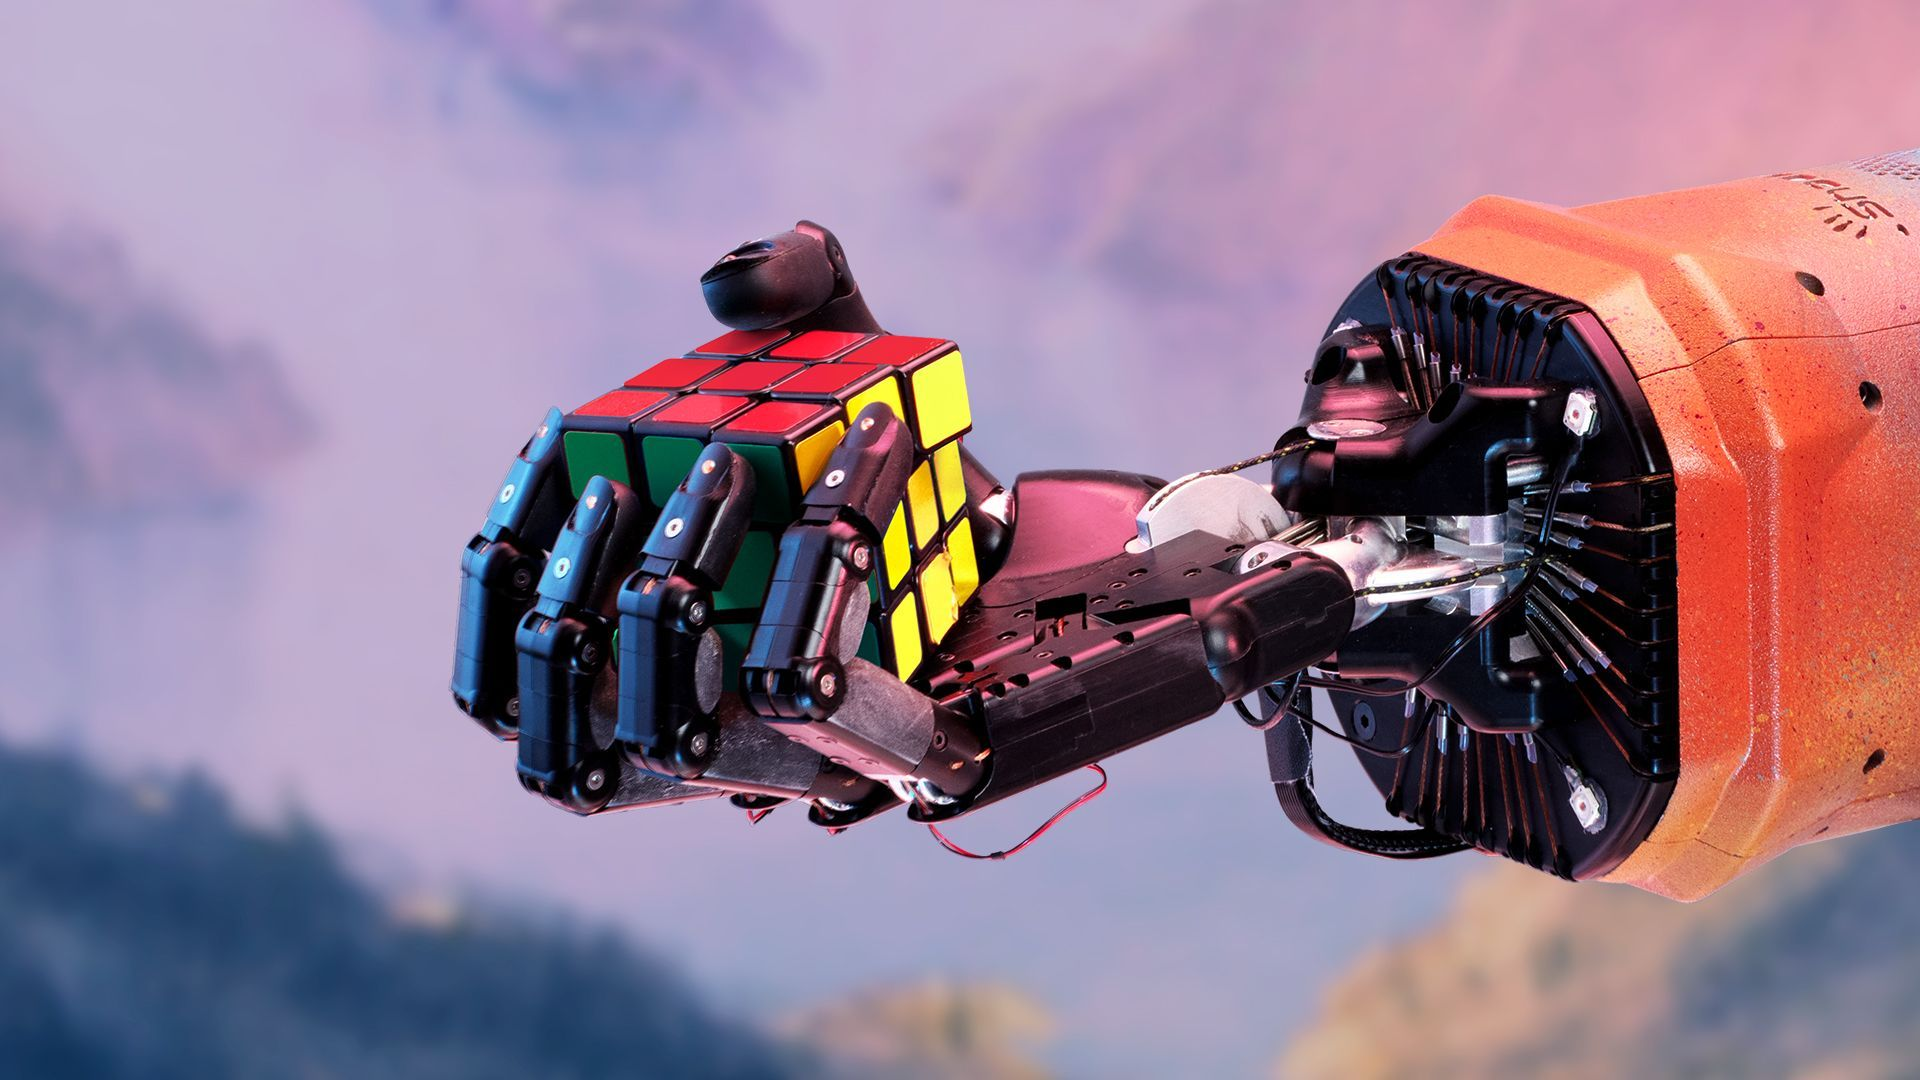
\includegraphics[keepaspectratio,width=\textwidth]{assets/openai_rubiks}

    \caption{\footfullcite{openai2019solving}}
  \end{figure}
\end{frame}

\begin{frame}{Deep RL Successes}
  \begin{figure}
    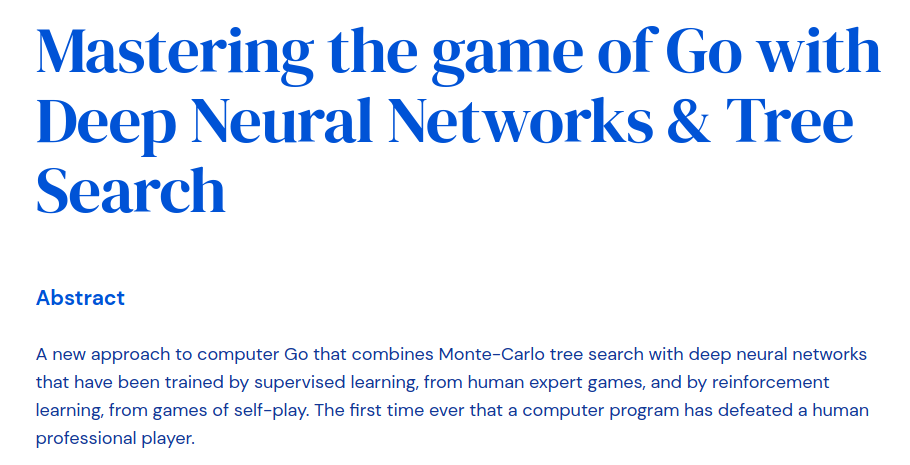
\includegraphics[keepaspectratio,width=\textwidth]{assets/alphago}
  \end{figure}
\end{frame}

\begin{frame}{Does Deep RL Really Work?}
  My previous work suggests not really, at least for control.
  \begin{figure}
    \subfigure[Joint Layout]{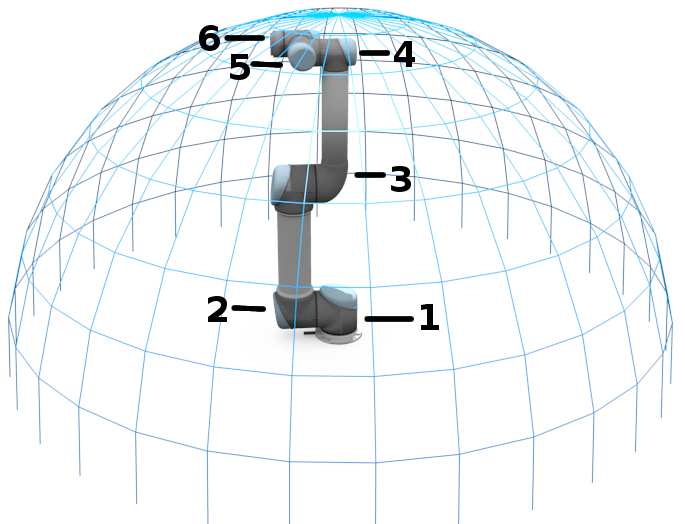
\includegraphics[width=0.32\linewidth]{assets/joint_viz}}
    \subfigure[1--2]{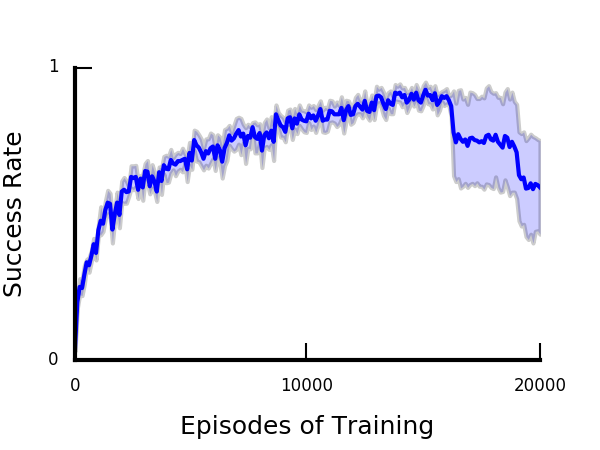
\includegraphics[width=0.32\linewidth]{assets/2joint_unconstrained}}
    \subfigure[1--3]{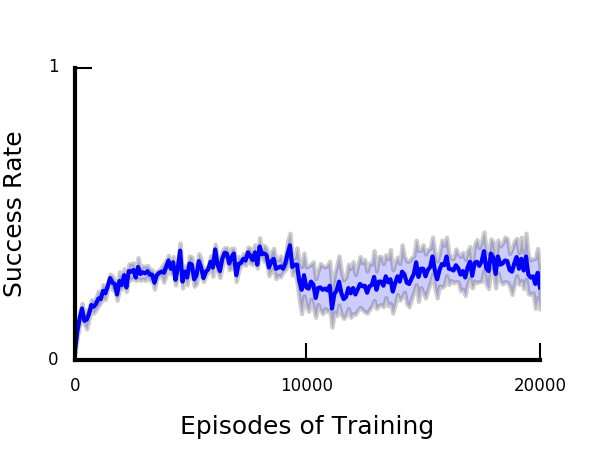
\includegraphics[width=0.32\linewidth]{assets/3joint_unconstrained}}
    \subfigure[1--4]{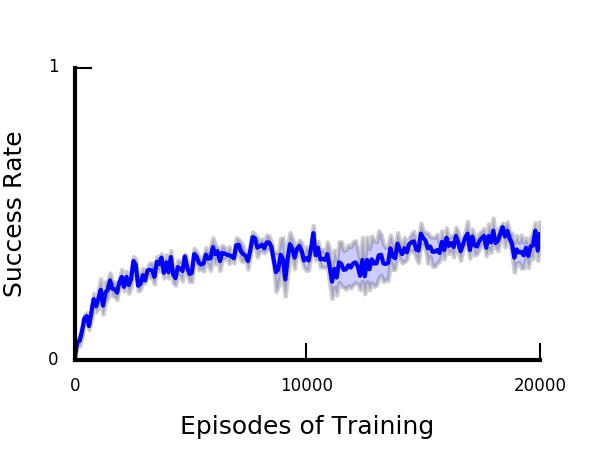
\includegraphics[width=0.32\linewidth]{assets/4joint_unconstrained}}
    \subfigure[1--5]{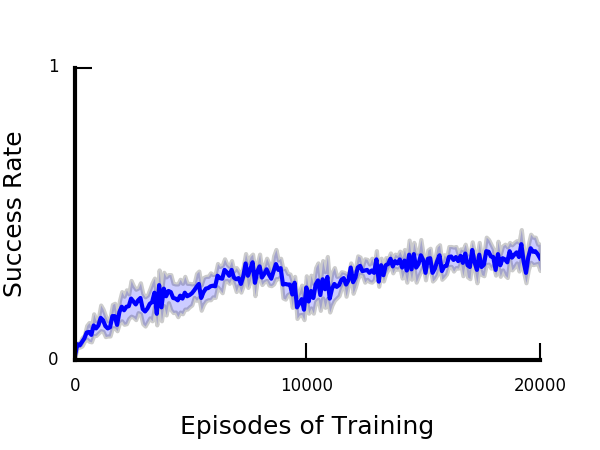
\includegraphics[width=0.32\linewidth]{assets/5joint_unconstrained}}
    \subfigure[1--6]{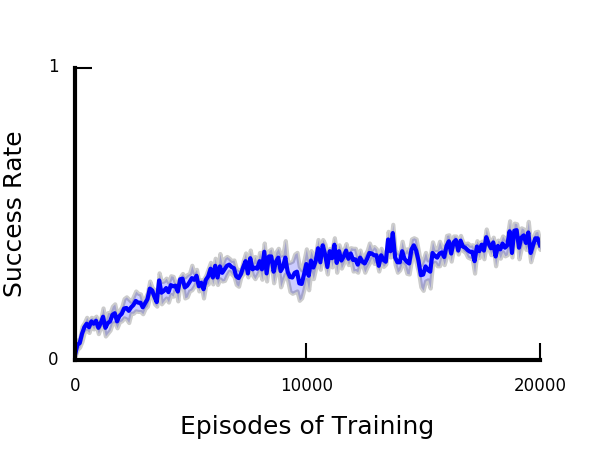
\includegraphics[width=0.32\linewidth]{assets/6joint_unconstrained}}
  \end{figure}
\end{frame}

\begin{frame}{Deep RL Data Hunger}
  \begin{itemize}
    \item Companies (DeepMind, OpenAI, etc.) using incredible amounts of compute
    \item The OpenAI Rubik's cube result took \emph{13,000 years} of simulated time
    \item It's clearly infeasible to run these algorithms on real robots
  \end{itemize}
\end{frame}

\begin{frame}{Safety \& Interpretability}
  \begin{itemize}
    \item We need to \textbf{verify safety} of controllers
    \item We can't even interpret neural networks for supervised learning
    \item Would you trust an uncertified neural network to fly a helicopter?
  \end{itemize}
\end{frame}

\end{document}
